\documentclass{beamer}

\usepackage[T1,T2A]{fontenc}
\usepackage[utf8]{inputenc}
\usepackage[english,russian]{babel}
\usepackage{textcomp}
\usepackage[normalem]{ulem}
\usepackage{hyperref} 

\usetheme{Madrid}

\usepackage{graphicx}

\usepackage{xcolor}
\definecolor{bluekeywords}{rgb}{0,0,1}
\definecolor{greencomments}{rgb}{0,0.5,0}
\definecolor{redstrings}{rgb}{0.64,0.08,0.08}
\definecolor{xmlcomments}{rgb}{0.5,0.5,0.5}
\definecolor{types}{rgb}{0.17,0.57,0.68}

\usepackage{listings}
\lstset{
language=[Sharp]C, 
showspaces=false,
showtabs=false,
breaklines=true,
showstringspaces=false,
breakatwhitespace=true,
escapeinside={(*@}{@*)},
morekeywords={partial, var, value, get, set, async, await, Task},
commentstyle=\color{greencomments},
keywordstyle=\color{bluekeywords},
stringstyle=\color{redstrings},
basicstyle=\ttfamily\small
}

\AtBeginSection[]{
  \begin{frame}
  \vfill
  \centering
  \begin{beamercolorbox}[sep=8pt,center,shadow=true,rounded=true]{title}
    \usebeamerfont{title}\insertsectionhead\par%
  \end{beamercolorbox}
  \vfill
  \end{frame}
}

\title{HttpClient} 
\subtitle{прошлое, настоящее, будущее}
\author{Риваль Абдрахманов}
\institute[PT]{Positive Technologies} 
\date{SpbDotNet, 2019}

\begin{document}
\begin{frame}
\titlepage
\end{frame}

\begin{frame}
\frametitle{Содержание}
\tableofcontents
\end{frame}

\section{HttpClient - базовая информация}

\begin{frame}{\href{https://docs.microsoft.com/en-us/dotnet/api/system.net.http.httpclient?view=netcore-2.2}{HttpClient Class}}
    \begin{itemize}
        \item <1-> Provides a base class for sending HTTP requests and receiving HTTP responses from a resource identified by a URI;
        \item <2-> $GetAsync(\ldots)$, $PostAsync(\ldots)$, $SendAsync(\ldots)$ и др.;
        \item <3-> $HttpClient$ реализует $IDisposable$.
    \end{itemize}
\end{frame}

\begin{frame}{\href{https://docs.microsoft.com/en-us/dotnet/api/system.idisposable?view=netcore-2.2}{IDisposable Interface}}
    \begin{itemize}
        \item <1-> Provides a mechanism for releasing unmanaged resources;
        \item <2-> $public\,void\,Dispose()$;
        \item <3-> Конструкция $using(\ldots)$;
        \item <4-> Диспозиться\,\textrightarrow \,диспозь
    \end{itemize}
\end{frame}

\begin{frame}{\href{https://docs.microsoft.com/en-us/dotnet/api/system.idisposable?view=netcore-2.2}{IDisposable Interface}}
    \begin{itemize}
        \item Provides a mechanism for releasing unmanaged resources;
        \item $public\,void\,Dispose()$;
        \item Конструкция $using(\ldots)$;
        \item \sout{Диспозиться\,\textrightarrow \,диспозь}
        \item Диспозиться\,\textrightarrow \,внимательней
    \end{itemize}
\end{frame}

\begin{frame}[fragile]
\frametitle{Disposable HttpClient}
\begin{lstlisting}
using(var client = new HttpClient())
{
  var response = await client.GetStringAsync(...);
}
\end{lstlisting}
\end{frame}

\section{Неочевидные проблемы}
\begin{frame}
\frametitle{Проблема socket exhaustion}
\href{https://aspnetmonsters.com/2016/08/2016-08-27-httpclientwrong/}{https://aspnetmonsters.com/2016/08/2016-08-27-httpclientwrong/}
\begin{figure}
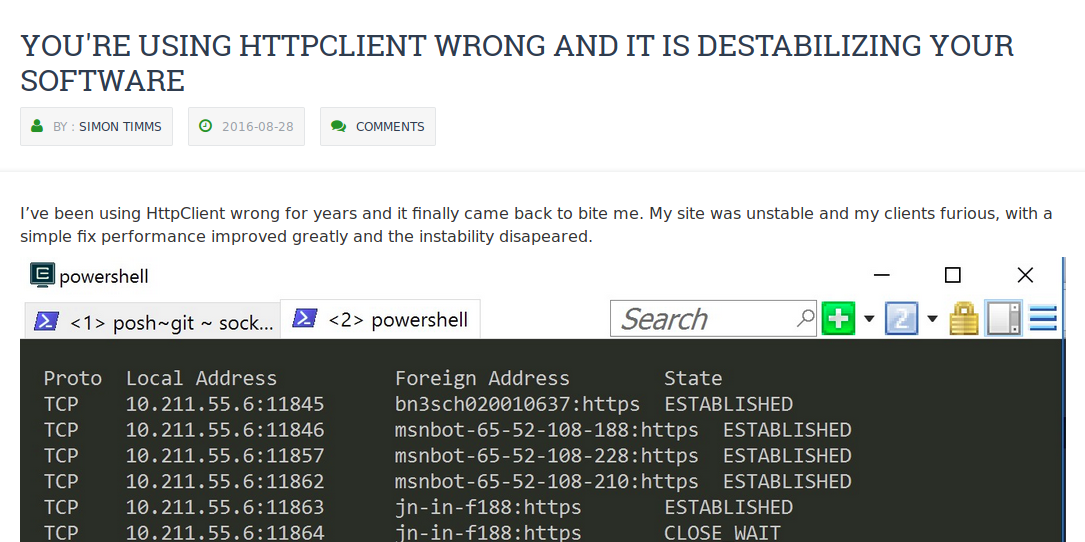
\includegraphics[scale=0.3]{aspnetmonsters}
\end{figure}
\end{frame}

\begin{frame}[fragile]
\frametitle{Проблема socket exhaustion}
\begin{lstlisting}
for(int i = 0; i < 10; i++)
{
  using (var client = new HttpClient())
  {
    await client.GetStringAsync("https://google.com");
  }
}
\end{lstlisting}
\end{frame}

\begin{frame}
\frametitle{Проблема socket exhaustion}
Проверяем через netstat:
\begin{figure}
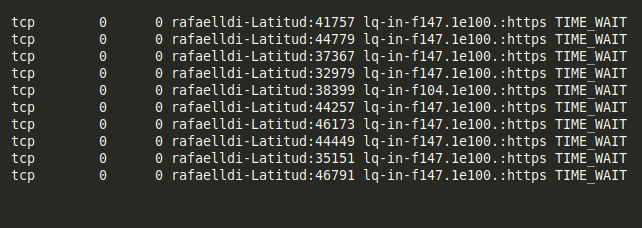
\includegraphics[scale=0.53]{netstat}
\end{figure}
\end{frame}

\begin{frame}
\frametitle{Проблема socket exhaustion}
\begin{itemize}
	\item 10 сокетов в состоянии \textit{TIME WAIT};
	\item Соединение закрыто с одной стороны, но мы всё ещё ждём доходящие пакеты, чтобы правильно их обработать;
	\item Приводит к $SocketException$.
\end{itemize}
\end{frame}

\begin{frame}
\frametitle{Проблема socket exhaustion}
``HttpClient is intended to be instantiated once and re-used throughout the life of an application. Instantiating an HttpClient class for every request will exhaust the number of sockets available under heavy loads.''
\newline
\newline
\textit{\href{https://docs.microsoft.com/en-us/dotnet/api/system.net.http.httpclient}{https://docs.microsoft.com/en-us/dotnet/api/system.net.http.httpclient}}
\end{frame}

\begin{frame}[fragile]
\frametitle{Проблема socket exhaustion}
Решение проблемы - переиспользование клиента:
\begin{lstlisting}
private static HttpClient Client = new HttpClient();
\end{lstlisting}
\end{frame}

\begin{frame}
\frametitle{Проблема кеширования DNS}
\href{https://byterot.blogspot.com/2016/07/singleton-httpclient-dns.html}{https://byterot.blogspot.com/2016/07/singleton-httpclient-dns.html}
\begin{figure}
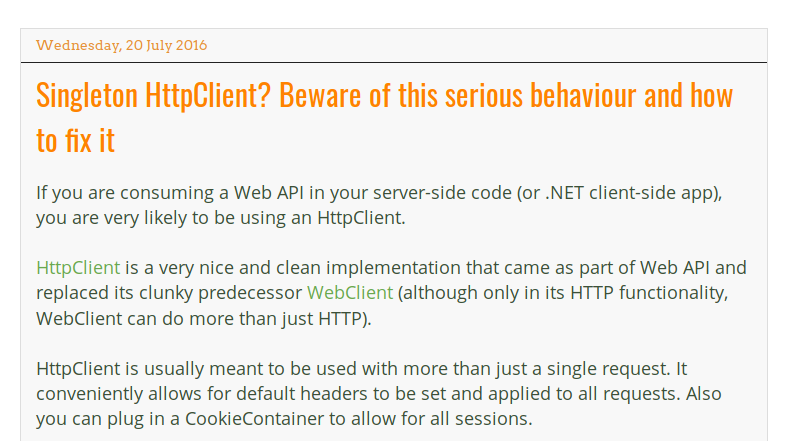
\includegraphics[scale=0.4]{byterot}
\end{figure}
\end{frame}

\begin{frame}
\frametitle{Проблема кеширования DNS}
\begin{itemize}
	\item Не учитываются изменения DNS;
	\item Соединение держится до закрытия сокета.
\end{itemize}
\end{frame}

\begin{frame}
\frametitle{Проблема кеширования DNS}
Решение для .NET Framework:
\begin{itemize}
	\item Класс $ServicePointManager$;
	\item $ServicePointManager.DnsRefreshTimeout$ -- время, которое будет закеширован полученный IP адрес для каждого доменного имени, по умолчанию 2 минуты;
	\item $ServicePoint.ConnectionLeaseTimeout$ -- время, которое соединение будет удерживаться открытым, по умолчанию не ограничено;
	\item $ServicePoint.MaxIdleTime$ -- время бездействия, после которого соединение будет закрыто.
\end{itemize}
\end{frame}

\begin{frame}[fragile]
\frametitle{Проблема кеширования DNS}
Пример:
\\
\begin{lstlisting}
ServicePointManager.DnsRefreshTimeout = 60000;

var sp = ServicePointManager.FindServicePoint(
  new Uri("https://google.com"));
sp.ConnectionLeaseTimeout = 60000;
sp.MaxIdleTime = 60000;
\end{lstlisting}
\end{frame}

\begin{frame}
\frametitle{Лимит одновременных соединений с сервером}
\href{https://habr.com/ru/post/424873/}{https://habr.com/ru/post/424873/}
\begin{figure}
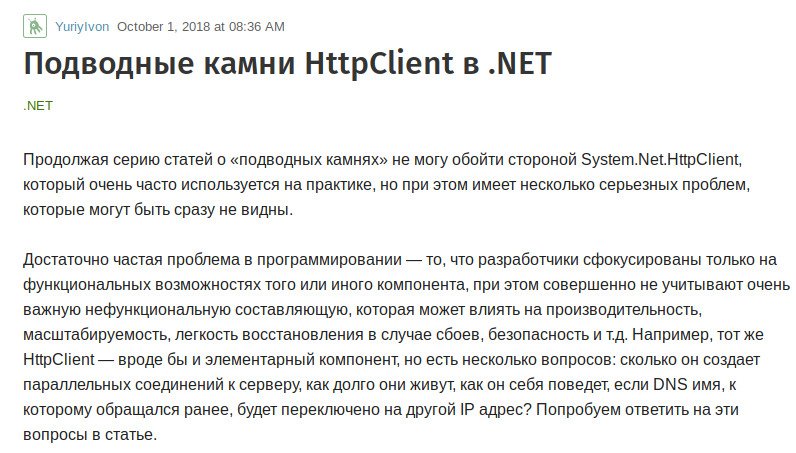
\includegraphics[scale=0.4]{habr}
\end{figure}
\end{frame}

\begin{frame}
\frametitle{Лимит одновременных соединений с сервером}
\begin{itemize}
	\item Лимит одновременных соединений с сервером по умолчанию равен 2;
	\item $ServicePointManager.DefaultConnectionLimit$;
	\item Для $localhost$ по умолчанию равен $int.MaxValue$;
	\item Только для .NET Framework.
\end{itemize}
\end{frame}

\section{Интерфейс IHttpClientFactory}
\begin{frame}
\frametitle{\href{https://docs.microsoft.com/en-us/dotnet/api/system.net.http.ihttpclientfactory?view=aspnetcore-2.2}{IHttpClientFactory}}
\begin{block}{IHttpClientFactory}
An IHttpClientFactory can be registered and used to configure and create HttpClient instances in an app.
\end{block}
Интерфейс был добавлен в ASP.NET Core 2.1.
\newline
\newline
Для консольного приложения придётся добавить \href{https://www.nuget.org/packages/Microsoft.Extensions.Hosting}{$Microsoft.Extensions.Hosting$} и \href{https://www.nuget.org/packages/Microsoft.Extensions.Http}{$Microsoft.Extensions.Http$}.
\end{frame}

\begin{frame}[fragile]
\frametitle{IHttpClientFactory - базовое использование}
\begin{itemize}
\item<1-> Регистрация через метод расширения $IServiceCollection$:
\begin{lstlisting}
services.AddHttpClient();
\end{lstlisting}
\item<2-> Добавление в конструктор с помощью DI:
\begin{lstlisting}
public SomeService(IHttpClientFactory clientFactory)
{
  _clientFactory = clientFactory;
}
\end{lstlisting}
\item<3-> Создание клиента (без $using$):
\begin{lstlisting}
var client = _clientFactory.CreateClient();
var response = await client.SendAsync(request);
\end{lstlisting}
\end{itemize}
\end{frame}

\begin{frame}[fragile]
\frametitle{Named clients}
\begin{itemize}
\item<1-> Регистрация через метод расширения $IServiceCollection$:
\begin{lstlisting}
services.AddHttpClient("some-site", c =>
{
  c.BaseAddress = 
    new Uri("https://some-site.com/");
  c.DefaultRequestHeaders
    .Add("Accept", "application/json");
});
\end{lstlisting}
\item<2-> Добавление в конструктор с помощью DI:
\begin{lstlisting}
public SomeService(IHttpClientFactory clientFactory)
{
  _clientFactory = clientFactory;
}
\end{lstlisting}
\item<3-> Создание клиента:
\begin{lstlisting}
var client = _clientFactory.CreateClient("some-site");
\end{lstlisting}
\end{itemize}
\end{frame}

\begin{frame}[fragile]
\frametitle{Typed clients}
Класс типизированного клиента:
\begin{lstlisting}
public class SomeSiteClient
{
  private readonly HttpClient _client;

  public SomeSiteClient(HttpClient client)
  {
    client.BaseAddress = 
      new Uri("https://some-site.com/");
    client.DefaultRequestHeaders
      .Add("Accept", "application/json");

    _client = client;
  }
    
  ...
}
\end{lstlisting}
\end{frame}

\begin{frame}[fragile]
\frametitle{Typed clients}
Класс типизированного клиента:
\begin{lstlisting}
public class SomeSiteClient
{
  ...

  public async Task<SomeData> GetSomeData()
  {
    var response = 
      await _client.GetAsync("/get-some-data");

    ...

    return result;
  }
}
\end{lstlisting}
\end{frame}

\begin{frame}[fragile]
\frametitle{Typed clients}
\begin{itemize}
\item<1-> Регистрация типизированного клиента:
\begin{lstlisting}
services.AddHttpClient<SomeSiteClient>();
\end{lstlisting}
\item<2-> Добавление в конструктор через DI:
\begin{lstlisting}
public SomeService(SomeSiteClient someSiteClient)
{
  _someSiteClient = someSiteClient;
}
\end{lstlisting}
\end{itemize}
\end{frame}

\begin{frame}[fragile]
\frametitle{Refit}
Библиотека Refit для REST API (\href{https://github.com/reactiveui/refit}{https://github.com/reactiveui/refit})
\newline
\begin{lstlisting}
public interface ISomeSiteClient
{
  [Get("/get-some-data")]
  Task<SomeData> GetSomeData();
}

public class SomeData
{
  public string Message { get; set; }
}
\end{lstlisting}
\end{frame}

\begin{frame}[fragile]
\frametitle{Refit}
\begin{itemize}
\item<1-> Регистрация клиента:
\begin{lstlisting}
services
  .AddRefitClient<ISomeSiteClient>()
  .ConfigureHttpClient(c => c.BaseAddress = 
    new Uri("https://some-site.com"));
\end{lstlisting}
\item<2-> Добавление в конструктор через DI:
\begin{lstlisting}
public SomeService(ISomeSiteClient someSiteClient)
{
  _someSiteClient = someSiteClient;
}
\end{lstlisting}
\end{itemize}
\end{frame}

\section{Дополнительные улучшения в .NET Core 2.1}
\begin{frame}
\frametitle{\href{https://docs.microsoft.com/en-us/dotnet/api/system.net.http.delegatinghandler?view=netcore-2.2}{DelegatingHandler}}
\begin{itemize}
\item $DelegatingHandler$ позволяют создать цепочку обработки исходящих запросов;
\item Схоже с middleware в ASP.NET Core;
\item Функциональность уже была, но с $IHttpClientFactory$ стало проще использовать.
\end{itemize}
\end{frame}

\begin{frame}[fragile]
\frametitle{Создание DelegatingHandler}
\begin{lstlisting}
public class SomeHandler : DelegatingHandler
{
  protected override async Task<HttpResponseMessage> SendAsync(HttpRequestMessage request, CancellationToken cancellationToken)
  {
    ...
        
    var response = await base.SendAsync(request, cancellationToken);

    ...
        
    return response;        
  }
}
\end{lstlisting}
\end{frame}

\begin{frame}[fragile]
\frametitle{Регистрация DelegatingHandler}
\begin{lstlisting}
services.AddHttpClient("some-site")
  //first
  .AddHttpMessageHandler<OutsideHandler>()
  //second
  .AddHttpMessageHandler<InsideHandler>()
\end{lstlisting}
\end{frame}

\begin{frame}
\frametitle{\href{https://github.com/App-vNext/Polly}{Polly}}
\begin{itemize}
\item \href{https://github.com/App-vNext/Polly}{Polly} - популярная библиотека обработки ошибок;
\item Содержит различные политики: Retry, Circuit Breaker, Timeout, \ldots
\item Необходимо установить \href{https://www.nuget.org/packages/Microsoft.Extensions.Http.Polly/}{$Microsoft.Extensions.Http.Polly$};
\item Подходит не только для $HttpClient$.
\end{itemize}
\begin{figure}

\includegraphics[scale=0.4]{polly}
\end{figure}
\end{frame}

\begin{frame}[fragile]
\frametitle{Добавление политик}
Обработка всех ответов со статус кодами 5xx и 408.
\newline
\begin{lstlisting}
services.AddHttpClient("some-site")
  .AddTransientHttpErrorPolicy(p => p.RetryAsync(3))
  .AddTransientHttpErrorPolicy(
    p => p.CircuitBreakerAsync(5, 
      TimeSpan.FromSeconds(30)));
\end{lstlisting}
\end{frame}

\begin{frame}[fragile]
\frametitle{Настройка внутреннего \href{https://docs.microsoft.com/en-us/dotnet/api/system.net.http.socketshttphandler?view=netcore-2.2}{HttpMessageHandler}}
\begin{lstlisting}
services.AddHttpClient("some-site")
  .ConfigurePrimaryHttpMessageHandler(() =>
  {
    return new SocketsHttpHandler()
    {
      AutomaticDecompression = 
        DecompressionMethods.GZip
    };
  });
\end{lstlisting}
\end{frame}

\begin{frame}[fragile]
\frametitle{Настройка времени жизни \href{https://docs.microsoft.com/en-us/dotnet/api/system.net.http.socketshttphandler?view=netcore-2.2}{HttpMessageHandler}}
\begin{itemize}
\item Для каждого именованного клиента есть свой $HttpMessageHandler$;
\item $IHttpClientFactory$ при создании нового $HttpClient$ будет переиспользовать $HttpMessageHandler$, если его время жизни не вышло;
\item Время жизни по умолчанию 2 минуты.
\end{itemize}
\begin{lstlisting}
services.AddHttpClient("some-site")
  .SetHandlerLifetime(TimeSpan.FromMinutes(5));
\end{lstlisting}
\end{frame}


\section{HttpRequestMessage и HttpResponseMessage}
\begin{frame}
\end{frame}

\section{Новое в .NET Core 3.0}
\begin{frame}
\end{frame}

\end{document}
